\chapter[Dise\~no]{
  \label{chp:diseno}
  DISE\~NO
}
\thispagestyle{numberingStyle}
\pagestyle{numberingStyle}


\section{Arquitectura del sistema}
La arquitectura empleada en nuestro sistema será una arquitectura en capas, una de las técnicas de diseño más usadas en las ciencias de la computación. La arquitectura basada en capas es una especialización de la arquitectura cliente-servidor donde la carga de trabajo se divide en diferentes capas con un reparto claro de las funciones.

En la arquitectura basada en capas, una capa inferior proporciona un servicio a otra copa superior. El servicio ofrecido se define mediante un contrato de servicio. De esta forma, se consigue independizar el software de ambas capas y los cambios de implementación en una de ellas, no tiene repercusión sobre las demás capas.

Partiendo de que la aplicación será accesible desde dispositivo móvil y navegador web, se presentará dos alternativas diferentes, en lo referente a la distribución de las capas, según el cliente empleado. 


\subsection{Arquitectura en 3 capas}



\subsection{Arquitectura en 4 capas}
Para el diseño de la aplicación accesible mediante navegador, se emplea una arquitectura en 4 capas.

\begin{figure}[!h]

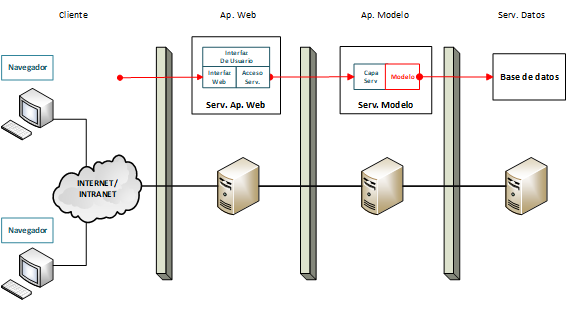
\includegraphics[
   keepaspectratio=true
]{./05_Diseno/arq4capas.png}
\caption{Diagrama arquitectura en cuatro capas}
\end{figure}


\subsection{Arquitectura completa del sistema}



\section{Capa Modelo}
\subsection{Diagrama clases persistentes}
\subsection{Diseño módulo acceso a datos}
\subsection{Diseño módulo servicios}
\section{Capa servicio REST}
\section{Controlador}
\subsection{Aplicación web}
\subsection{Aplicación móvil}

\section{Diseño físco de los datos}
\subsection{Modelo Entidad-Relación}
\subsection{Modelo Relacional}






